\chapter{\ifproject%
\ifenglish Experimentation and Results\else การทดลองและผลลัพธ์\fi
\else%
\ifenglish System Evaluation\else การประเมินระบบ\fi
\fi}

\hspace{10mm} เนื่องจากมีการนำความรู้เรื่อง Computer Vision มาใช้เกี่ยวกับการทำ Object detection จึงได้มีการศึกษา model และ library
ของ OpenCV ที่มีให้ทดลองใช้งาน เพื่อเพิ่มความเข้าใจและเลือกใช้ได้อย่างเหมาะสม โดยนำภาพบางส่วนจากการถ่ายรูปสถานที่จริงด้วยกล้องโทรศัพท์มือถือคือบริเวณชั้น 2
ของสำนักหอสมุดมหาวิทยาลัยเชียงใหม่มาทำการทดสอบ

\begin{figure}[h]
    \centering
    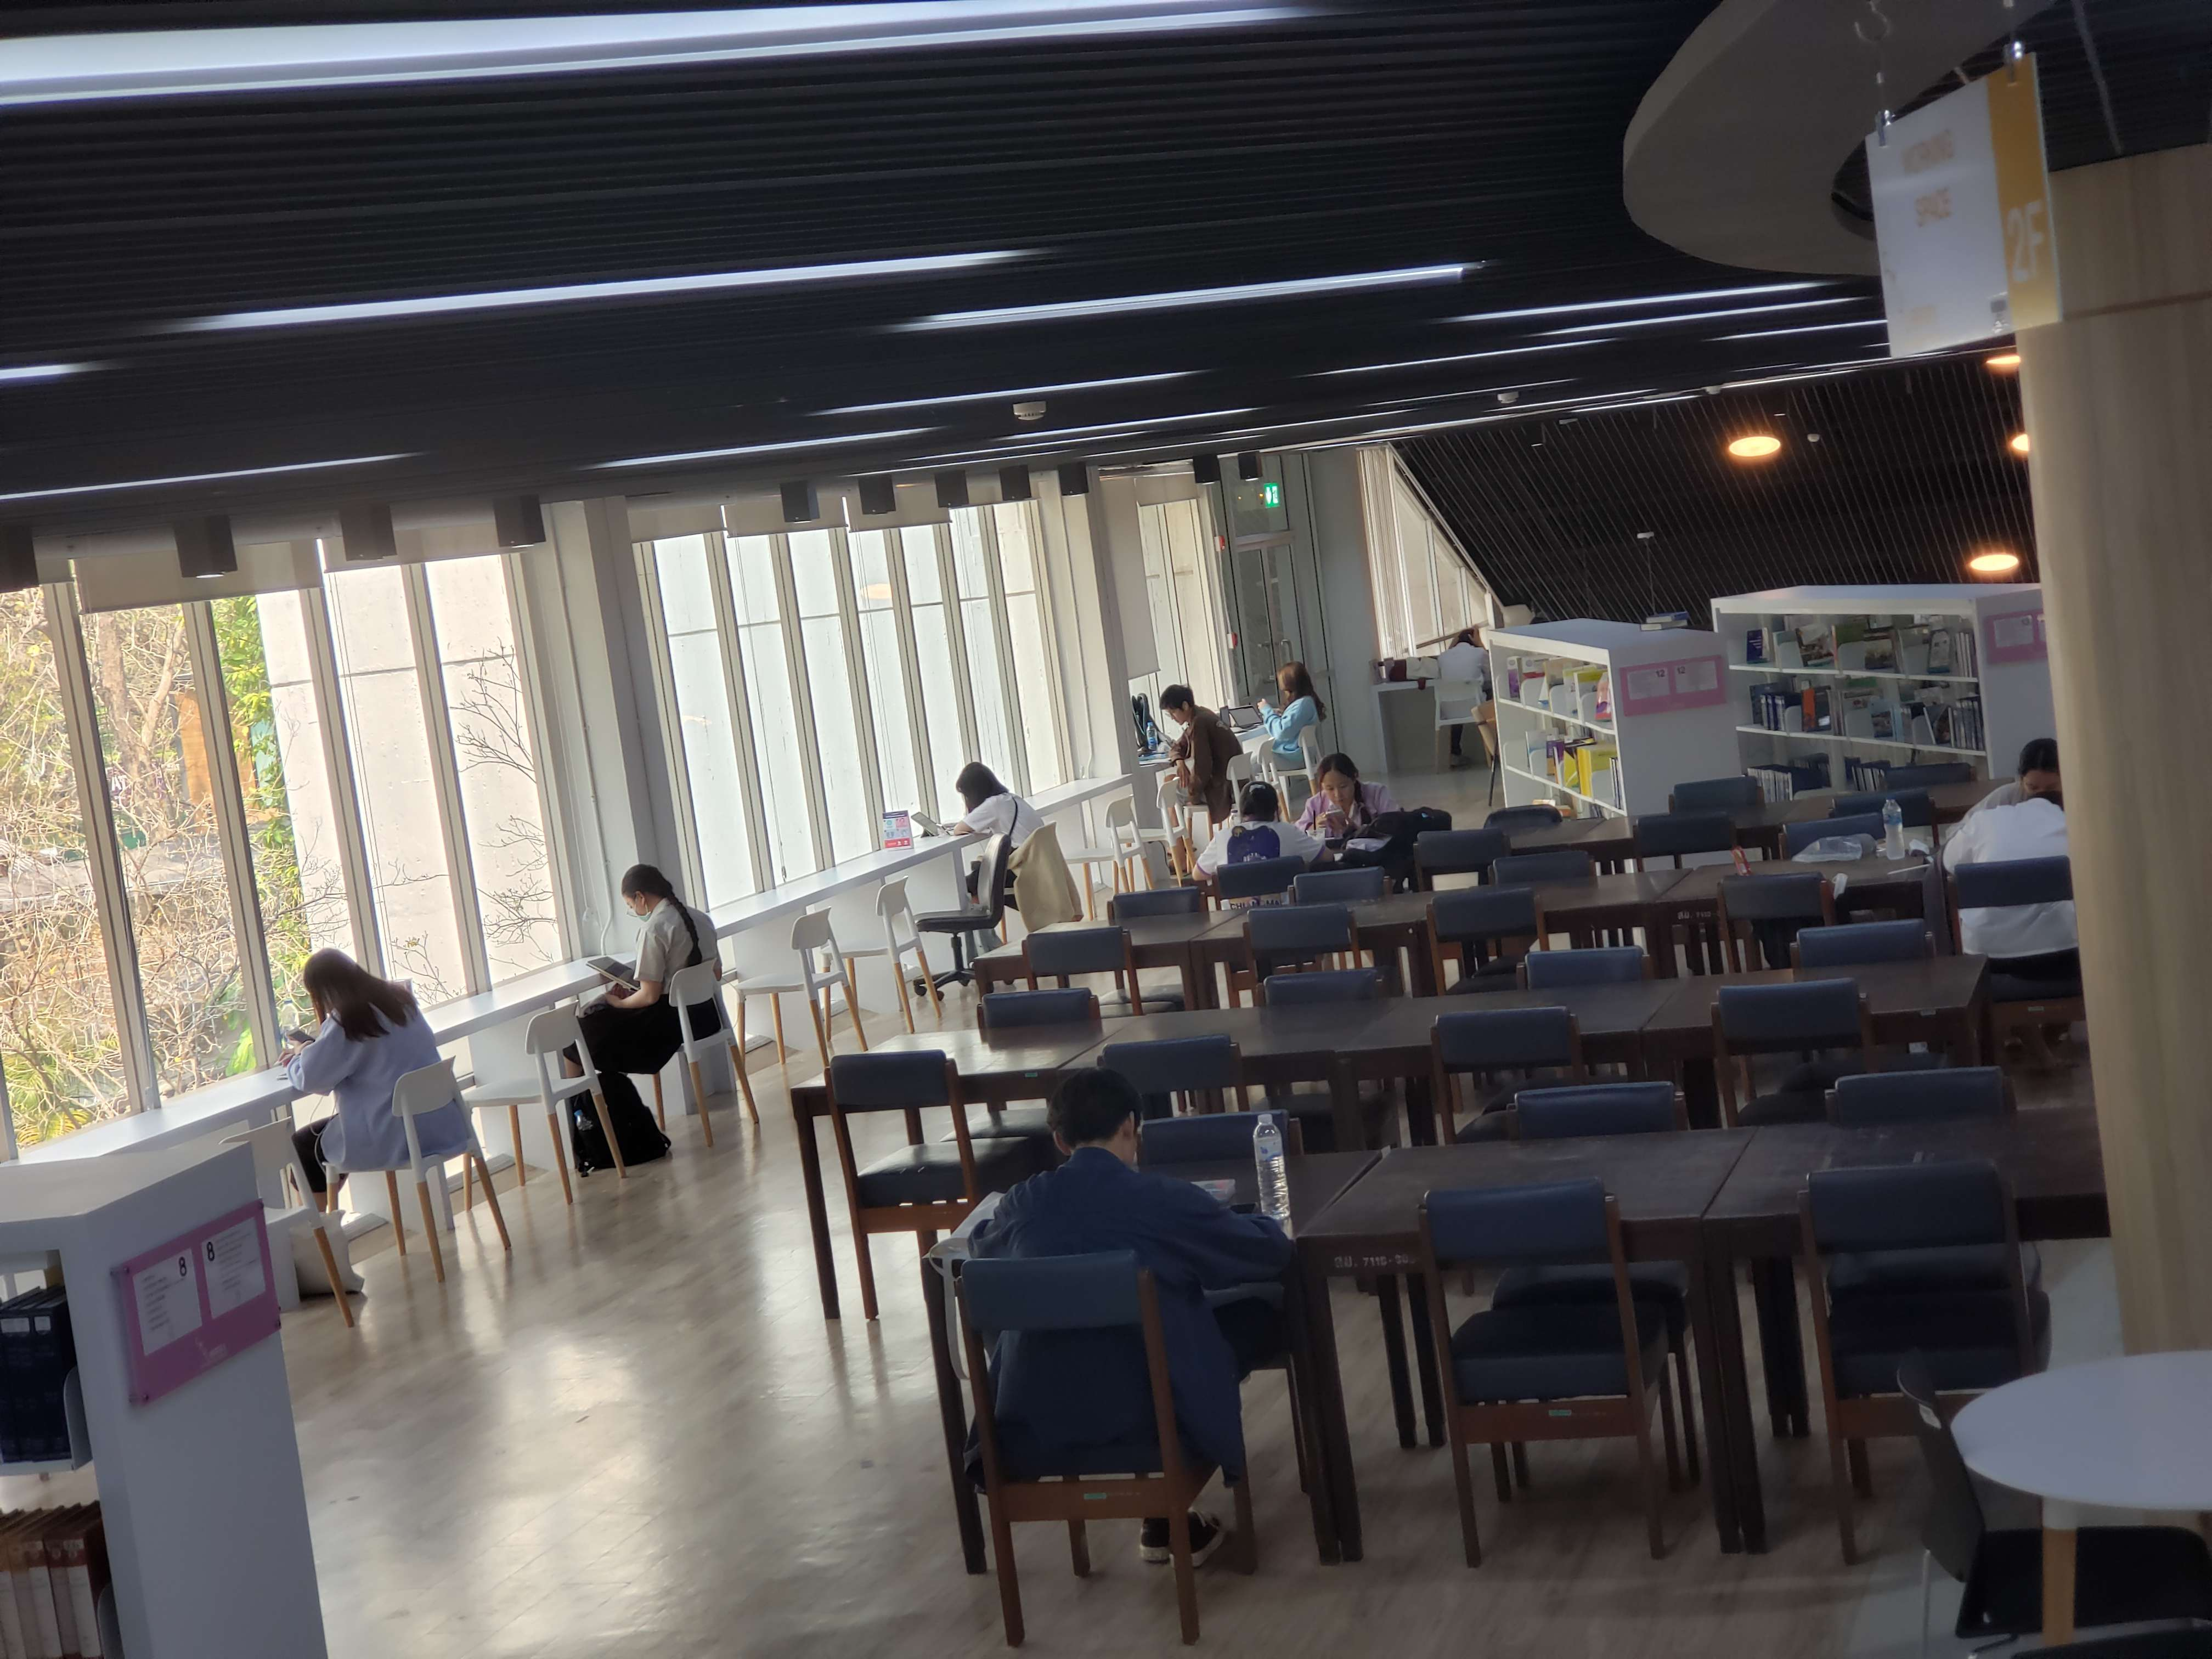
\includegraphics[scale=0.07]{images/cam2-2.jpg}
    \caption[camera]{ภาพจากกล้องโทรศัพท์มือถือ}
    \label{fig:camera}
\end{figure}

\section{การทดลองครั้งที่ 1 โดยใช้ OpenCV with HOG descriptor}
\begin{figure}[ht]
\centering
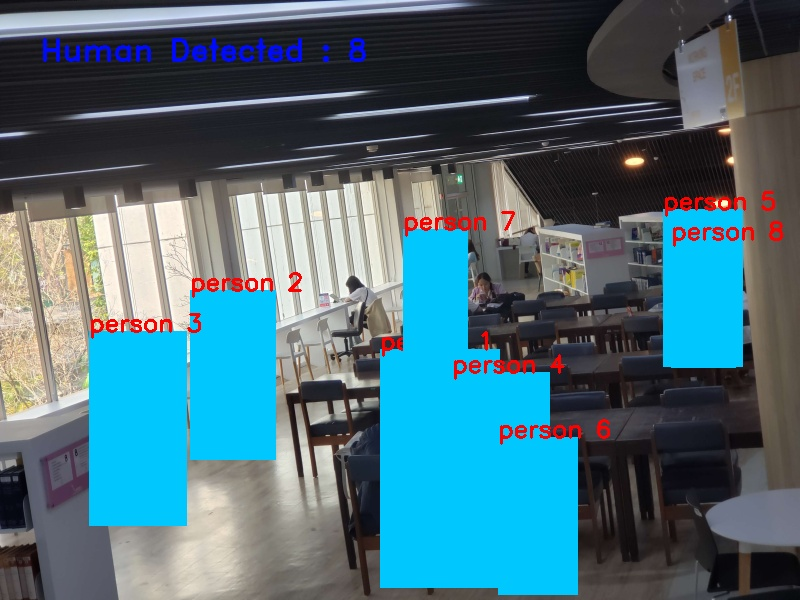
\includegraphics[scale=0.35]{images/hog_output.jpg}
\caption[output1]{output ของการทดลองครั้งที่ 1}
\label{fig:output1}
\end{figure}

\section{การทดลองครั้งที่ 2 โดยใช้ OpenCV with Detect common object library}
\begin{figure}[ht]
\centering
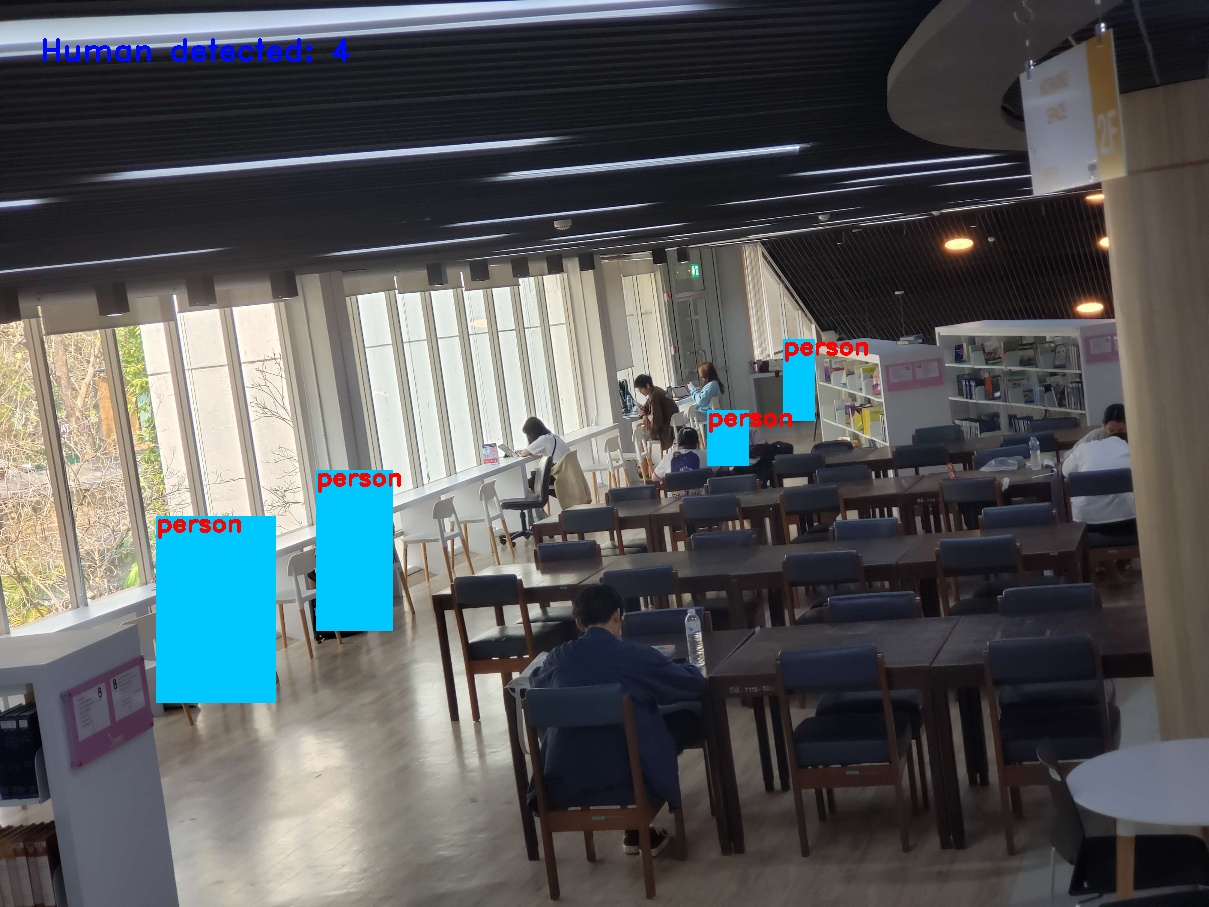
\includegraphics[scale=0.25]{images/cvlib_output.jpg}
\caption[output2]{output ของการทดลองครั้งที่ 2}
\label{fig:output2}
\end{figure}

\section{การทดลองครั้งที่ 3 โดยใช้ OpenCV DNN with TensorFlow}
\begin{figure}[ht]
\centering
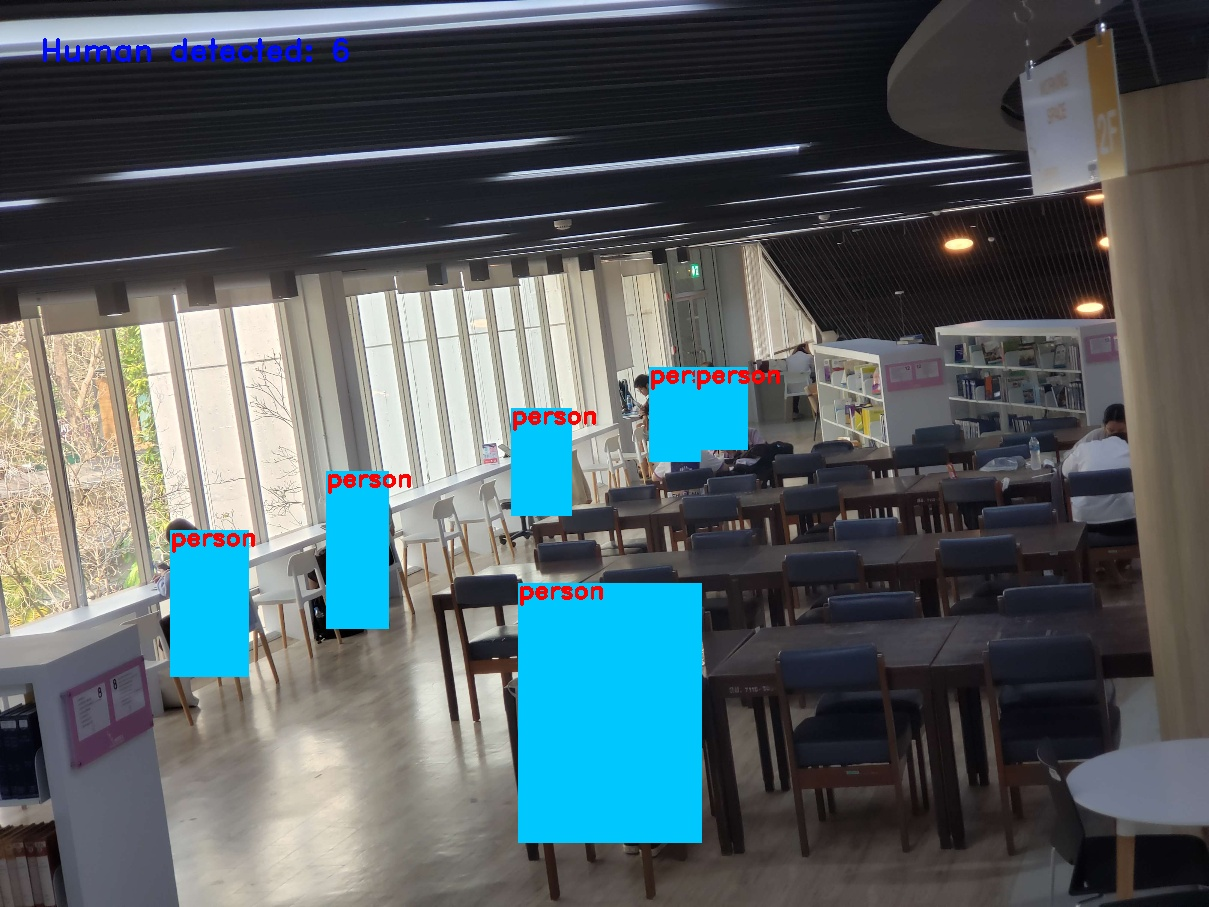
\includegraphics[scale=0.25]{images/dnn_output.jpg}
\caption[output3]{output ของการทดลองครั้งที่ 3}
\label{fig:output3}
\end{figure}
